% Number 60
% Vectors Relv
% Relative velocity - sailboat/wind
% MIT Physics for Teachers LON-CAPA

% Watermark
\AddToShipoutPicture*{\BackgroundPic}

\addtocounter {ProbNum} {1}

\begin{floatingfigure}[r]{.35\textwidth}
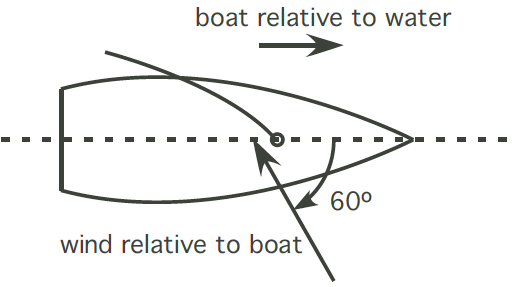
\includegraphics[scale=.4]{/Users/jgates/desktop/latex/pics/sailboat1.png}
\end{floatingfigure}
 
{\bf \Large{\arabic{ProbNum}}} A sailboat is moving forward at a speed of 5 knots relative to the water. A gauge attached to its mast indicates a wind speed of 10 knots at an angle of 60 degrees, both relative to the boat. 
\bigskip

\indent What is the wind speed relative to the water?

\vfill

\newpage
